\documentclass[
	11pt,
	oneside,
	openany,
	french,
	onehalfspacing,
	liststotoc,
	toctotoc,
	parskip,
	headsepline,
	consistentlayout,
]{template}

\usepackage{babel}
\usepackage[utf8]{inputenc}
\usepackage[T1]{fontenc}
\usepackage{emoji}
\usepackage{amsmath,amssymb}
\usepackage{newpxtext,newpxmath}
\usepackage{booktabs}

\usepackage[backend=biber,style=numeric,sortcites,natbib=true,sorting=none]{biblatex}
\addbibresource{example.bib}
\usepackage{graphicx,wrapfig}
\usepackage{pdflscape}
\usepackage{lipsum}
\usepackage{geometry}
\geometry{
	paper=a4paper,
	inner=2.5cm,
	outer=2.5cm,
	top=2.5cm,
	bottom=2.5cm,
}

\usepackage{float}
\usepackage{lipsum} % for filler text
\usepackage{listings}
\usepackage{courier}
\usepackage{pdflscape}




\thesistitle{\textsc{ \Huge{House Inventory \emoji{houses}} \\ \huge Conception et réalisation d’une application de gestion des stocks}}
\supervisor{M. El Mostafa \textsc{El Rhoudri} \\ M. Mahmoud \textsc{El Hamlaoui}}
\author{Badr-Eddine \textsc{Marani} \\ Badr-Eddine \textsc{Marani}}
\university{\href{http://www.centrale-casablanca.ma/}{Ecole Centrale Casablanca}}

\begin{document}
% 	\frontmatter
	\pagestyle{plain}
	\begin{titlepage}
		\begin{center}
			\vspace*{.06\textheight}
			{\scshape\LARGE \univname\par}\vspace{1.5cm}
			\textsc{\Large Rapport projet de base des données}\\[0.5cm]

			\HRule \\[0.4cm]
			{\huge \bfseries \ttitle\par}\vspace{0.4cm}
			\HRule \\[1.5cm]

			\begin{minipage}[t]{0.4\textwidth}
				\begin{flushleft} \large
					\emph{Réalisé par :}\\
					\href{mailto:badr-eddine.marani@centrale-casablanca.ma}{Badr-Eddine \textsc{Marani}}

					\href{mailto:aymen.lakhyar@centrale-casablanca.ma}{Aymen \textsc{Lakhyar}}
				\end{flushleft}
			\end{minipage}
			\begin{minipage}[t]{0.4\textwidth}
				\begin{flushright} \large
					\emph{Encadrants :} \\
					\href{}{Prof. Mahmoud \textsc{El Hamlaoui}}

					\href{}{Prof. Abderrahim \textsc{Ait Wakrime}}


				\end{flushright}
			\end{minipage}\\[3cm]


			\Large Ce rapport est soumis dans le cadre du projet de base de données.\\[0.3cm]

			\vspace*{\fill}

			{\large Année académique 2021 -- 2022}\\[4cm]
		\end{center}
	\end{titlepage}

	\tableofcontents

	\listoffigures

	\listoftables

	\chapter{Introduction générale} \label{Chapter1}

\section{Présentation de projet}
Dans le cadre de la formation d’ingénieur de l’École Centrale Casablanca, les élèves de deuxième année doivent réaliser un projet base de données. Celui-ci consiste sur une durée de deux mois avec une fréquence d’une séance par semaine, à conceptualiser et réaliser un système de gestion d’une base de données.
C’est dans cette optique que nous avons eu le plaisir de choisir le thème : système d'inventaire de maison.

Aujourd'hui, les logiciels sont utilisés dans presque tous les domaines de la vie quotidienne. Les téléphones portables, les télévisions, les appareils de chauffage, les voitures et même certains de nos grille-pains sont dotés de logiciels qui les rendent plus faciles à utiliser et améliorent ainsi la vie des personnes qui les utilisent.  Avec l'arrivée de cette nouvelle technologie dans nos voitures et nos téléphones portables, il semble étrange que l'endroit où nous passons le plus de temps soit à la traîne dans cette tendance. Nos maisons sont désormais la prochaine facette de notre vie que nous devrions améliorer.

\begin{figure}[ht]
    \centering
    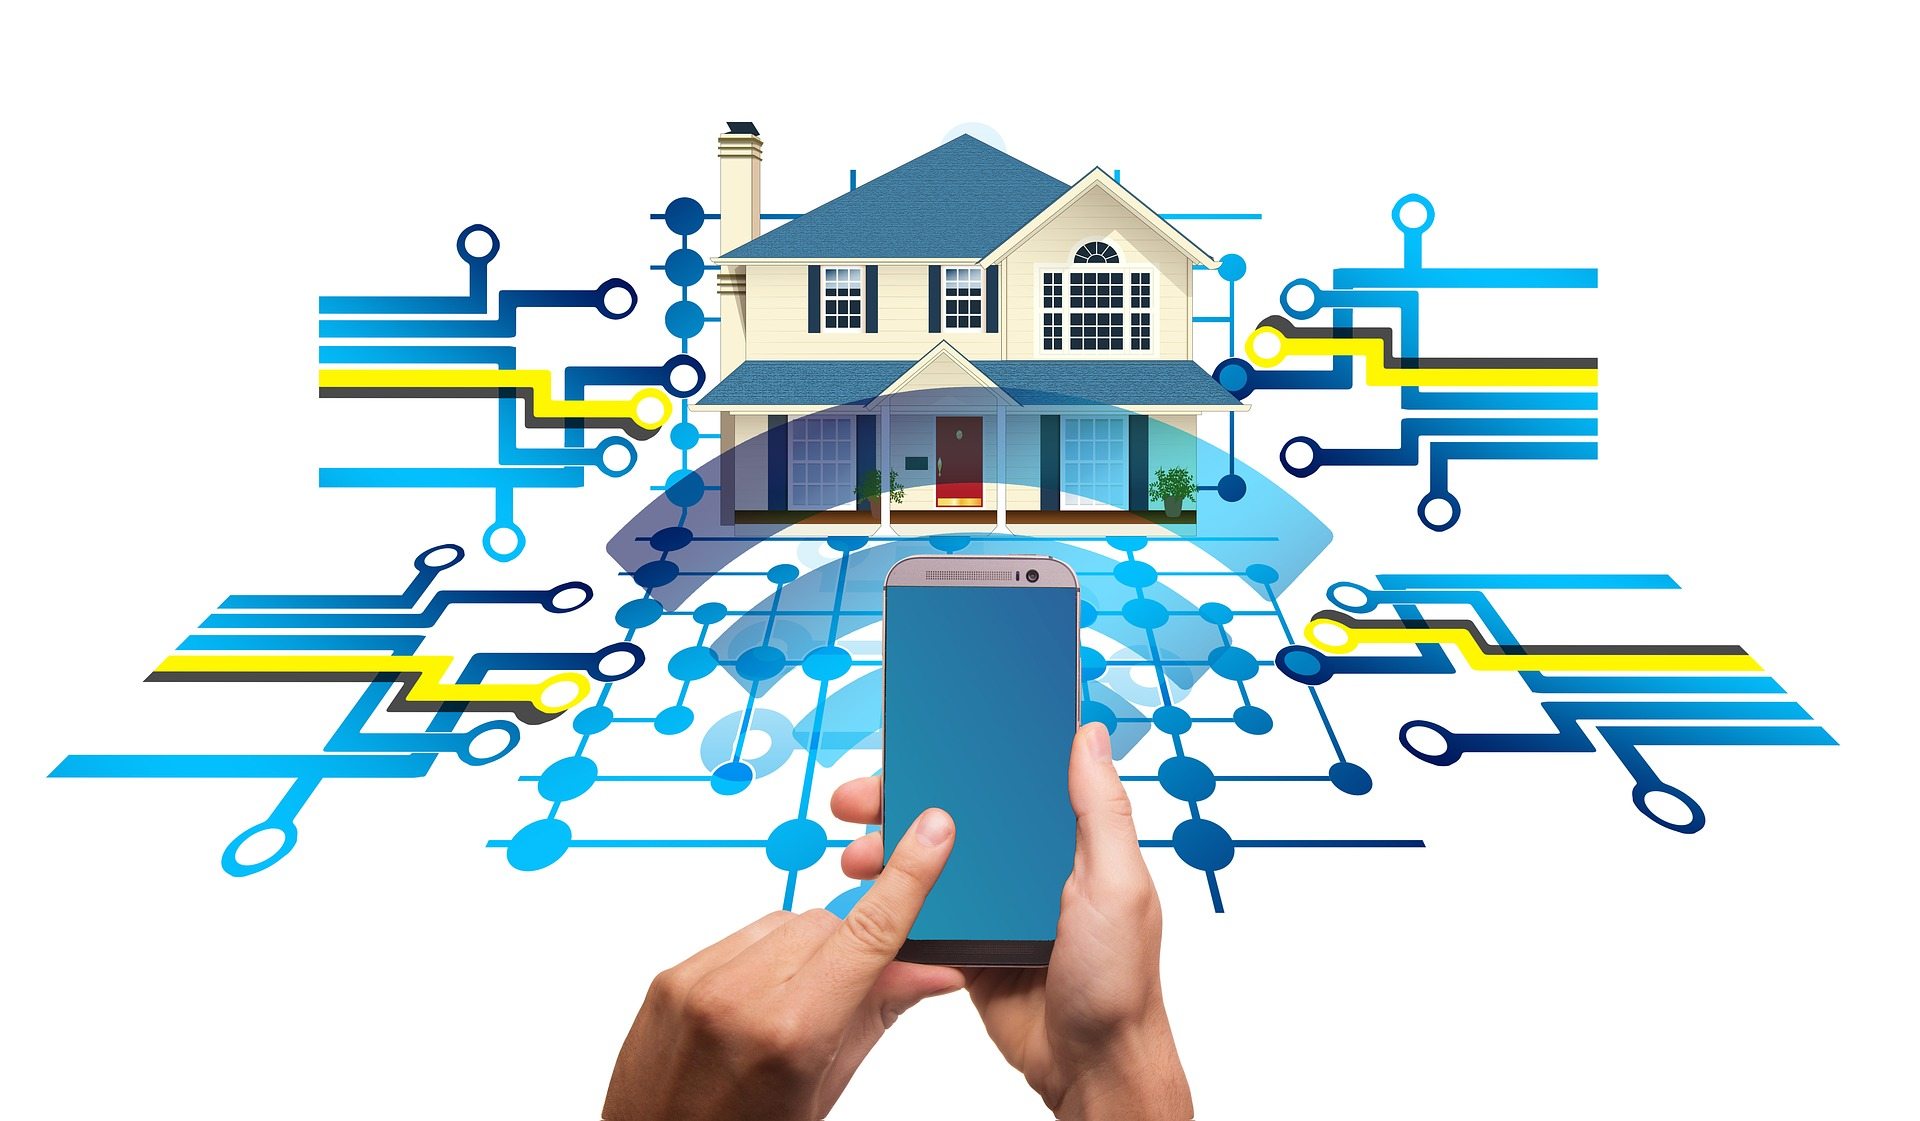
\includegraphics[keepaspectratio=true,scale=0.65]{Figures/smart-home.jpg}
    \caption{Smart Home}
    \label{fig:structure}
\end{figure}

La "Smart Home" est une maison qui utilise les nouvelles technologies pour faciliter la vie de ses occupants. Que vous soyez une personne âgée vivant seule ou un étudiant, chacun peut les utiliser. Avant de pouvoir construire une véritable maison intelligente, nous devons développer les composants qui constitueront la base du système. L'un de ces composants, d'une importance vitale, est un moyen d'organiser et de garder la trace des objets de la maison. Le système d’inventaire de maison est une idée simple qui peut être utilisée comme l'un des composants de la maison intelligente. Imaginez qu'un terrible accident détruise la maison d'un particulier ; il arrive souvent que le compte exact des biens personnels du propriétaire devienne un problème entre lui et la compagnie d'assurance. L'inventaire de la maison résout ce problème en gardant la trace de chaque objet de la maison, ce qui simplifie considérablement le recouvrement des pertes en cas d'accident.

Dans la suite de ce rapport, nous exposerons tous les résultats que nous avons obtenus à l’issu de ce projet.

\section{Plan de travail}
\subsection{Organisation du rapport}
Le rapport est divisé en cinq chapitres principaux décrivant le projet, les processus et les résultats, voir figure \ref{fig:structure}. Le premier chapitre est une introduction au projet. La deuxième partie consiste en une étude préalable sur la méthode que nous allons utiliser, les exigences des utilisateurs ( les exigences sont en gros divisées en deux groupes : les exigences fonctionnelles et les exigences non fonctionnelles ). Le troisième chapitre décrit la première phase du projet qui consiste à réaliser différents diagrammes (dictionnaire des données, MCD, et MLD). Le quatrième chapitre de ce rapport présente le prototype final, une présentation du prototype qui a été développé à partir des résultats identifiés et classés par ordre de priorité.  Pour conclure ce rapport, un dernier chapitre représentant la discussion et la conclusion du rapport est présenté.

\begin{figure}[ht]
    \centering
    
\includegraphics[keepaspectratio=true,scale=0.65]{Figures/structure-rapport.pdf}
    \caption{Structure du rapport}
    \label{fig:structure}
\end{figure}

\subsection{Diagramme de Gantt}
Tout au long de semestre, notre groupe a organisé des réunions, pendant lesquelles plusieurs aspects de la solution sont discutés. Les différentes composantes de notre produit final ont été choisi par le groupe, après plusieurs recherches. Le tableau et le diagramme Gant ci-dessous montrent les étapes de réalisation du prototype.

\begin{figure}[ht]
    \centering
    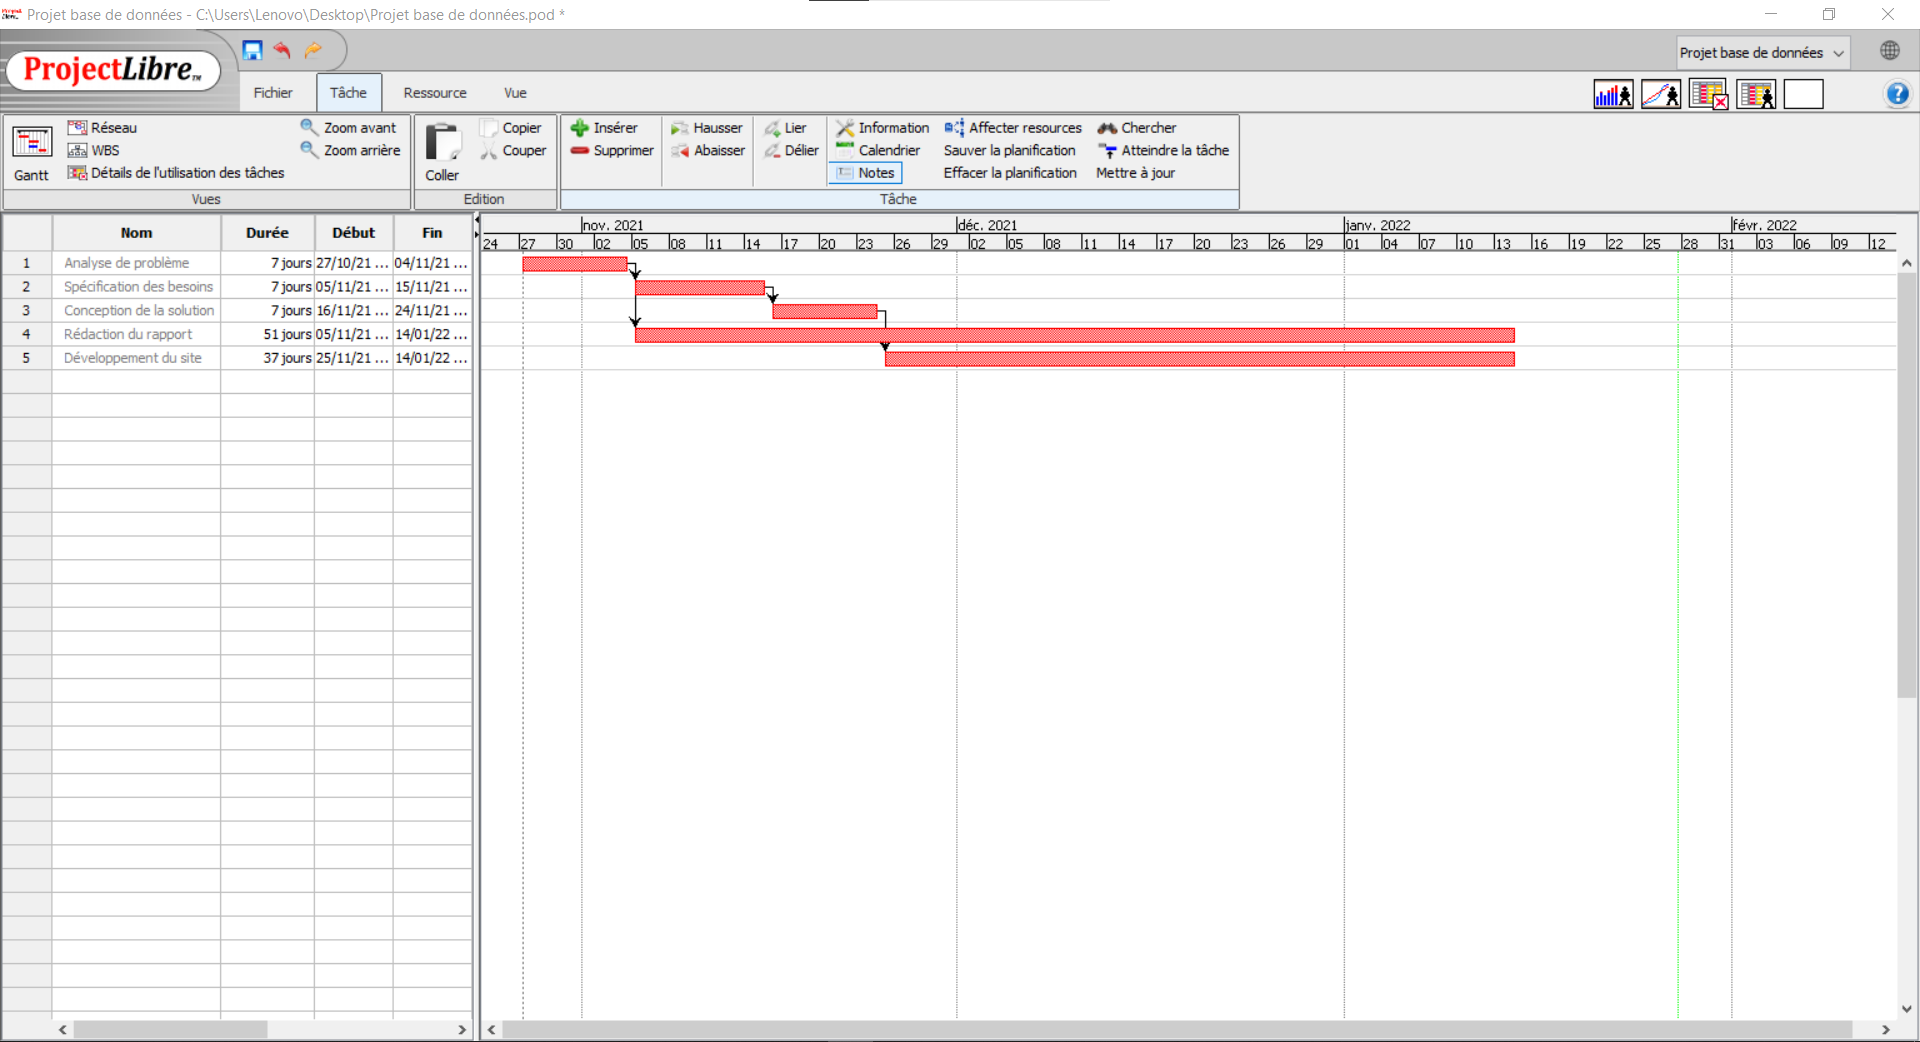
\includegraphics[keepaspectratio=true,scale=.6, angle = -90]{Figures/gantt.png}
    \caption{Diagramme de Gantt}
    \label{fig:structure}
\end{figure}

	\chapter{Étude préalable} \label{Chapter2}

\section{Méthode d’analyse et de conception : Merise}
Une méthode est la mise en œuvre de plusieurs étapes (méthodologiques), d'une démarche, de principes, d'outils.

La méthode MERISE est pour cela une méthodologie qui propose des étapes pour la mise en place et la conduite de projets informatiques. Le terme MERISE, acronyme signifiant méthode d'études et de réalisations de systèmes informatiques pour les entreprises, est le plus couramment et le plus largement utilisé pour la conception et la réalisation de bases de données en France.
Cette méthode vise à remplacer le système de gestion manuelle d'une organisation par un système automatisé de traitement de l'information. Elle vise, d'une part, à démontrer les problèmes potentiels du système existant et, d'autre part, à apporter des améliorations à ce dernier. Les facteurs considérés dans l'étude sont la collecte, le stockage, le traitement et la transmission de l'information.

\begin{figure}[ht!]
    \centering
    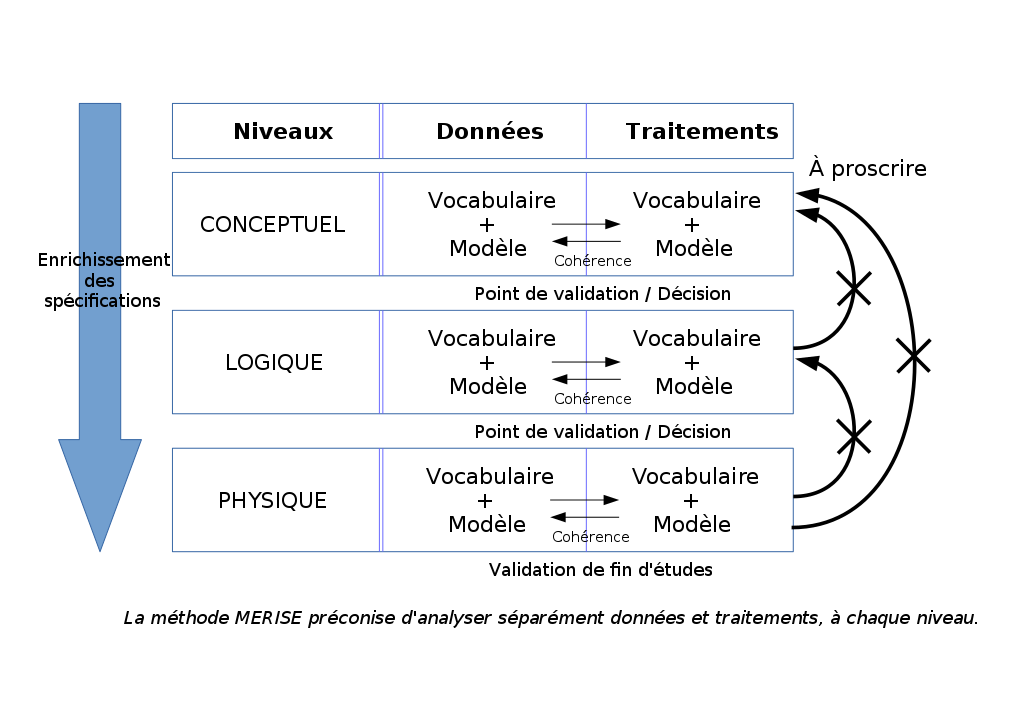
\includegraphics[keepaspectratio=true,scale=0.3]{Figures/merise.png}
    \caption{Méthode MERISE}
    \label{fig:merise}
\end{figure}

Ainsi, MERISE permet d'entreprendre une étude de l'existant et de passer à la conception proprement dite, si cette dernière est la solution, en procédant par exemple comme suit :

\paragraph{Étude de l'existant :} Ici on décrit de manière détaillée la structure existante qui décrit la situation réelle de l'organisation et son fonctionnement.
\paragraph{Analyse et évaluation de l'existant :} Identification des problèmes et des moyens de les résoudre.
\paragraph{Conception et mise en place du nouveau système :} proposer un modèle qui aboutit à la base de données ou encore proposer des interfaces et des programmes en utilisant certains langages de programmation et systèmes de gestion de bases de données.


Toutes ces étapes peuvent être résumées dans la figure \ref{fig:merise}.


\section{Analyse du problème}
\subsection{Contexte}
Le but est d'améliorer la gestion des stocks d’une maison. On va créer une application pour gérer efficacement leurs inventaires. Cette application permettra de gérer à la fois les articles achetés, et les produits, mais aussi de gérer l'inventaire hebdomadaire des lots par les dirigeants. Nous avons donc créé le cahier des charges suivant, qui décrit notre démarche.

\subsection{Analyse et aboutissements}
Pour des raisons de simplicité, on considère que les \textbf{produits} que nous stockerons dans la base de données sont tous des produits destinés uniquement à être consommés (viande, fruit, etc..).

Chaque produit a un identifiant, un libellé et une brève description, et chacun d'eux appartient à une \textbf{catégorie} spécifique. Il est possible de définir des caractéristiques communes entre certains produits. Ces caractéristiques communes peuvent être divisées en deux groupes : le premier est lié à la \textbf{forme} du produit (poids, hauteur, volume), et le second contient des \textbf{informations} générales telles que la date d'expiration, le prix unitaire, la quantité, et la température (minimale et maximale). Cet inventaire est créé indépendamment pour chaque utilisateur afin que les données de chacun soient séparées de celles des autres.

Chaque produit doit être inscrit à l'inventaire de la maison (\textbf{stock}). Il a un identifiant, un nom et la quantité de produit disponible. Il est acheté auprès d'une ou plusieurs entreprises à la fois. Ici, nous considérons que l'\textbf{entreprise} ne vend qu'un seul type de produits. Une entreprise peut être présente dans plus d'une \textbf{ville}. Ainsi, une ville peut contenir plusieurs entreprises.

Quand un \textbf{utilisateur} achète un nouveau produit ou augmente la quantité d'un produit. Nous le mettons dans le stock. Chaque produit comporte la date à laquelle il a été ajouté, ainsi qu'une date à laquelle nous le récupérons, au cas où il serait périmé ou que nous ne l'aurions plus en stock.

Chaque fois qu'un produit est ajouté au stock, l'utilisateur peut effectuer un \textbf{contrôle} pour vérifier si le produit est périmé ou non. L'utilisateur peut également vérifier, de temps en temps, la disponibilité d'un certain produit.

Chaque processus de contrôle doit être suivi d'une brève description de ses résultats. Bien évidemment, les résultats de ces contrôles peuvent être variés. Mais, pour simplifier, nous ne considérons dans ce projet que ces résultats typiques : produit périmé, produit non disponible en stock, produit disponible en stock.

\subsection{Fonctionnalités}

\paragraph{Parcourir les articles :} L'utilisateur parcourt les articles disponibles dans son inventaire.
\paragraph{Insérer un élément :} L'utilisateur insère un élément dans son inventaire.
\paragraph{Supprimer un élément :} L'utilisateur supprime un élément de l'inventaire.
\paragraph{Modifier l'élément :} L'utilisateur peut modifier les propriétés d'un élément.
\paragraph{Login :} Se connecter au système.
\paragraph{Logout :} Se déconnecter du système
\paragraph{Modifier l'identifiant et le mot de passe :} L'utilisateur peut changer son identifiant et son mot de passe.

\section{L’identification des besoins}
\subsection{Les besoins fonctionnels}
Le système doit assurer les fonctionnalités suivantes :

\paragraph{1. Le système doit permettre aux utilisateurs de modifier leurs mots de passe par mesure de sécurité.}
\paragraph{2. Le système doit permettre aux utilisateurs d'enregistrer toutes les informations relatives aux produits achetés, à ceux qui restent dans le stock.}
\paragraph{3. Le système doit être capable d'exporter tous les enregistrements stockés afin de les analyser.}

\subsection{Les besoins non fonctionnels}
\paragraph{Ergonomie et Convivialité}
L’application devra offrir aux utilisateurs un cadre de travail organiser et harmonieux. Par des interfaces graphiques claires et lisibles, la possibilité d’effectuer des recherches facilement, et de sauvegarder leurs données.

\paragraph{Facilité d’utilisation et facteur humain}
Nous voulons faciliter l’utilisation de l’application en simplifiant d’abord sa manipulation, ensuite en proposant un guide d’utilisation précis, afin qu’il soit utilisable par n’importe quel agriculteur. Aucune compétence en informatique ne sera nécessaire pour manipuler ce produit. L’utilisateur aura un accès à un menu "aide" où il pourra s’informer sur l’application, et communiquer ses difficultés ou préoccupations rencontrées.

\paragraph{Sécurité}
Chaque utilisateur aura un compte privé et un mot de passe qu’il devra fournir pour accéder au site, et ce mot de passe pourra au besoin être modifier pour assurer plus de sécurité.

\paragraph{Le système ne doit pas occuper plus que l'espace requis pour un programme normal à l'espace disque.}


\section{L’analyse des besoins : Identification des acteurs}
L'application sera généralement utilisée par deux types d'utilisateurs, un utilisateur à domicile et un administrateur système. Les utilisateurs à domicile sont des personnes qui utilisent le système pour leur inventaire quotidien. Les administrateurs du système constituent un groupe très restreint d'utilisateurs qui ont accès à l'ensemble du système et peuvent en modifier tous ses aspects.

% \section{Conclusion}

	\chapter{Conception} \label{Chapter3}

\section{Dictionnaire de données}

\begin{table}[ht!]
\centering
\resizebox{\columnwidth}{!}{%
\begin{tabular}{c|lllcl|}
\cline{2-6}
\multicolumn{1}{l|}{} &
  \multicolumn{5}{c|}{{\color[HTML]{000000} \textbf{Dictionnaire de données}}} \\ \cline{2-6}
\multicolumn{1}{l|}{} &
  \multicolumn{1}{c|}{\textbf{Nom symbolique}} &
  \multicolumn{1}{c|}{\textbf{Signification}} &
  \multicolumn{1}{c|}{\textbf{Type}} &
  \multicolumn{1}{c|}{\textbf{Taille}} &
  \multicolumn{1}{c|}{\textbf{Contraintes, règles de calcul}} \\ \hline
\multicolumn{1}{|c|}{} &
  \multicolumn{1}{l|}{{\ul \textbf{user\_id}}} &
  \multicolumn{1}{l|}{ID d'utilisateur} &
  \multicolumn{1}{l|}{Numérique} &
  \multicolumn{1}{c|}{100} &
  Automatique \\
\multicolumn{1}{|c|}{} &
  \multicolumn{1}{l|}{user\_nom} &
  \multicolumn{1}{l|}{Nom de l'utilisateur} &
  \multicolumn{1}{l|}{Alphanumérique} &
  \multicolumn{1}{c|}{50} &
  Obligatoire \\
\multicolumn{1}{|c|}{} &
  \multicolumn{1}{l|}{user\_email} &
  \multicolumn{1}{l|}{Adresse mail utilisateur} &
  \multicolumn{1}{l|}{Alphanumérique} &
  \multicolumn{1}{c|}{50} &
   \\
\multicolumn{1}{|c|}{} &
  \multicolumn{1}{l|}{user\_password} &
  \multicolumn{1}{l|}{Mot de passe utilisateur} &
  \multicolumn{1}{l|}{Alphanumérique} &
  \multicolumn{1}{c|}{50} &
  Obligatoire \\
\multicolumn{1}{|c|}{\multirow{}{}{\textbf{Utilisateur}}} &
  \multicolumn{1}{l|}{user\_derniere\_session} &
  \multicolumn{1}{l|}{Dernière sessios} &
  \multicolumn{1}{l|}{Date} &
  \multicolumn{1}{c|}{8} &
  Forme JJ-MM-AAAA \\ \hline
\multicolumn{1}{|c|}{} &
  \multicolumn{1}{l|}{{\ul \textbf{produit\_id}}} &
  \multicolumn{1}{l|}{ID produit} &
  \multicolumn{1}{l|}{Numérique} &
  \multicolumn{1}{c|}{100} &
  Automatique \\
\multicolumn{1}{|c|}{} &
  \multicolumn{1}{l|}{libelle\_produit} &
  \multicolumn{1}{l|}{Libellé produit} &
  \multicolumn{1}{l|}{Alphanumérique} &
  \multicolumn{1}{c|}{50} &
  Obligatoire \\
\multicolumn{1}{|c|}{} &
  \multicolumn{1}{l|}{produit\_temperature\_max} &
  \multicolumn{1}{l|}{Température maximal} &
  \multicolumn{1}{l|}{Numérique} &
  \multicolumn{1}{c|}{100} &
  Obligatoire, \textgreater 0 \\
\multicolumn{1}{|c|}{} &
  \multicolumn{1}{l|}{produit\_temperature\_min} &
  \multicolumn{1}{l|}{Température minimal} &
  \multicolumn{1}{l|}{Numérique} &
  \multicolumn{1}{c|}{100} &
  Obligatoire, \textgreater 0 \\
\multicolumn{1}{|c|}{\multirow{}{}{\textbf{Produit}}} &
  \multicolumn{1}{l|}{produit\_description} &
  \multicolumn{1}{l|}{Description du produit} &
  \multicolumn{1}{l|}{Alphanumérique} &
  \multicolumn{1}{c|}{100} &
  Obligatoire \\ \hline
\multicolumn{1}{|c|}{} &
  \multicolumn{1}{l|}{{\ul \textbf{catégorie\_id}}} &
  \multicolumn{1}{l|}{ID du catégorie} &
  \multicolumn{1}{l|}{Numérique} &
  \multicolumn{1}{c|}{100} &
  Automatique \\
\multicolumn{1}{|c|}{\multirow{}{}{\textbf{Catégorie}}} &
  \multicolumn{1}{l|}{libelle\_catégorie} &
  \multicolumn{1}{l|}{Libellé catégorie} &
  \multicolumn{1}{l|}{Alphanumérique} &
  \multicolumn{1}{c|}{50} &
  Obligatoire \\ \hline
\multicolumn{1}{|c|}{} &
  \multicolumn{1}{l|}{{\ul \textbf{taille\_id}}} &
  \multicolumn{1}{l|}{ID taille} &
  \multicolumn{1}{l|}{Numérique} &
  \multicolumn{1}{c|}{100} &
  Automatique \\
\multicolumn{1}{|c|}{} &
  \multicolumn{1}{l|}{libelle\_taille} &
  \multicolumn{1}{l|}{Libellé de la taille} &
  \multicolumn{1}{l|}{Numérique} &
  \multicolumn{1}{c|}{100} &
  Obligatoire, \textgreater 0 \\
\multicolumn{1}{|c|}{} &
  \multicolumn{1}{l|}{taille\_hauteur} &
  \multicolumn{1}{l|}{Hauteur du produit} &
  \multicolumn{1}{l|}{Numérique} &
  \multicolumn{1}{c|}{100} &
  Obligatoire, \textgreater 0 \\
\multicolumn{1}{|c|}{} &
  \multicolumn{1}{l|}{taille\_largeur} &
  \multicolumn{1}{l|}{Largeur du produit} &
  \multicolumn{1}{l|}{Numérique} &
  \multicolumn{1}{c|}{100} &
  Obligatoire, \textgreater 0 \\
\multicolumn{1}{|c|}{\multirow{}{}{\textbf{Taille}}} &
  \multicolumn{1}{l|}{volume} &
  \multicolumn{1}{l|}{Volume du produit} &
  \multicolumn{1}{l|}{Numérique} &
  \multicolumn{1}{c|}{100} &
  Obligatoire, \textgreater 0 \\ \hline
\multicolumn{1}{|c|}{} &
  \multicolumn{1}{l|}{{\ul \textbf{information\_id}}} &
  \multicolumn{1}{l|}{ID information} &
  \multicolumn{1}{l|}{Numérique} &
  \multicolumn{1}{c|}{100} &
  Automatique \\
\multicolumn{1}{|c|}{} &
  \multicolumn{1}{l|}{date\_expiration} &
  \multicolumn{1}{l|}{Date d'expiration du produit} &
  \multicolumn{1}{l|}{Date} &
  \multicolumn{1}{c|}{8} &
  Forme JJ-MM-AAAA \\
\multicolumn{1}{|c|}{} &
  \multicolumn{1}{l|}{date\_d\_arrivée} &
  \multicolumn{1}{l|}{Date d'arrivée du produit} &
  \multicolumn{1}{l|}{Date} &
  \multicolumn{1}{c|}{8} &
  Forme JJ-MM-AAAA \\
\multicolumn{1}{|c|}{\multirow{}{}{\textbf{Information}}} &
  \multicolumn{1}{l|}{prix\_unité} &
  \multicolumn{1}{l|}{Prix unité} &
  \multicolumn{1}{l|}{Numérique} &
  \multicolumn{1}{c|}{100} &
  Obligatoire, \textgreater 0 \\ \hline
\multicolumn{1}{|c|}{} &
  \multicolumn{1}{l|}{{\ul \textbf{entreprise\_id}}} &
  \multicolumn{1}{l|}{ID entreprise} &
  \multicolumn{1}{l|}{Numérique} &
  \multicolumn{1}{c|}{100} &
  Automatique \\
\multicolumn{1}{|c|}{} &
  \multicolumn{1}{l|}{entreprise\_nom} &
  \multicolumn{1}{l|}{Nom d'entreprise} &
  \multicolumn{1}{l|}{Alphanumérique} &
  \multicolumn{1}{c|}{50} &
  Obligatoire \\
\multicolumn{1}{|c|}{} &
  \multicolumn{1}{l|}{entreprise\_email} &
  \multicolumn{1}{l|}{Adresse mail d'entreprise} &
  \multicolumn{1}{l|}{Alphanumérique} &
  \multicolumn{1}{c|}{50} &
   \\
\multicolumn{1}{|c|}{\multirow{}{}{\textbf{Entreprise}}} &
  \multicolumn{1}{l|}{entreprise\_description} &
  \multicolumn{1}{l|}{Description d'entreprise} &
  \multicolumn{1}{l|}{Alphanumérique} &
  \multicolumn{1}{c|}{100} &
   \\ \hline
\multicolumn{1}{|c|}{} &
  \multicolumn{1}{l|}{{\ul \textbf{code\_postale}}} &
  \multicolumn{1}{l|}{Code postale} &
  \multicolumn{1}{l|}{Numérique} &
  \multicolumn{1}{c|}{10} &
  Obligatoire / Contient au mois 6 chiffres \\
\multicolumn{1}{|c|}{\multirow{}{}{\textbf{Ville}}} &
  \multicolumn{1}{l|}{ville} &
  \multicolumn{1}{l|}{Nom du ville} &
  \multicolumn{1}{l|}{Alphanumérique} &
  \multicolumn{1}{c|}{50} &
  Obligatoire \\ \hline
\multicolumn{1}{|c|}{} &
  \multicolumn{1}{l|}{{\ul \textbf{contrôle\_id}}} &
  \multicolumn{1}{l|}{ID du contrôle} &
  \multicolumn{1}{l|}{Numérique} &
  \multicolumn{1}{c|}{100} &
  Automatique \\
\multicolumn{1}{|c|}{} &
  \multicolumn{1}{l|}{contrôle\_date} &
  \multicolumn{1}{l|}{Date du contrôle} &
  \multicolumn{1}{l|}{Date} &
  \multicolumn{1}{c|}{8} &
  Forme JJ-MM-AAAA \\
\multicolumn{1}{|c|}{\multirow{}{}{\textbf{Contrôle}}} &
  \multicolumn{1}{l|}{contrôle\_résultat} &
  \multicolumn{1}{l|}{Résultat du contrôle} &
  \multicolumn{1}{l|}{Alphanumérique} &
  \multicolumn{1}{c|}{100} &
  Obligatoire \\ \hline
\end{tabular}
}
\caption{Dictionnaire de données}
\end{table}


\section{Modèle conceptuel de données (MCD)}
\subsection{Modèle EA}
A l’aide de l’analyse effectuée, nous avons pu établir le schéma conceptuel ci-dessous.
\begin{figure}[ht!]
    \centering
    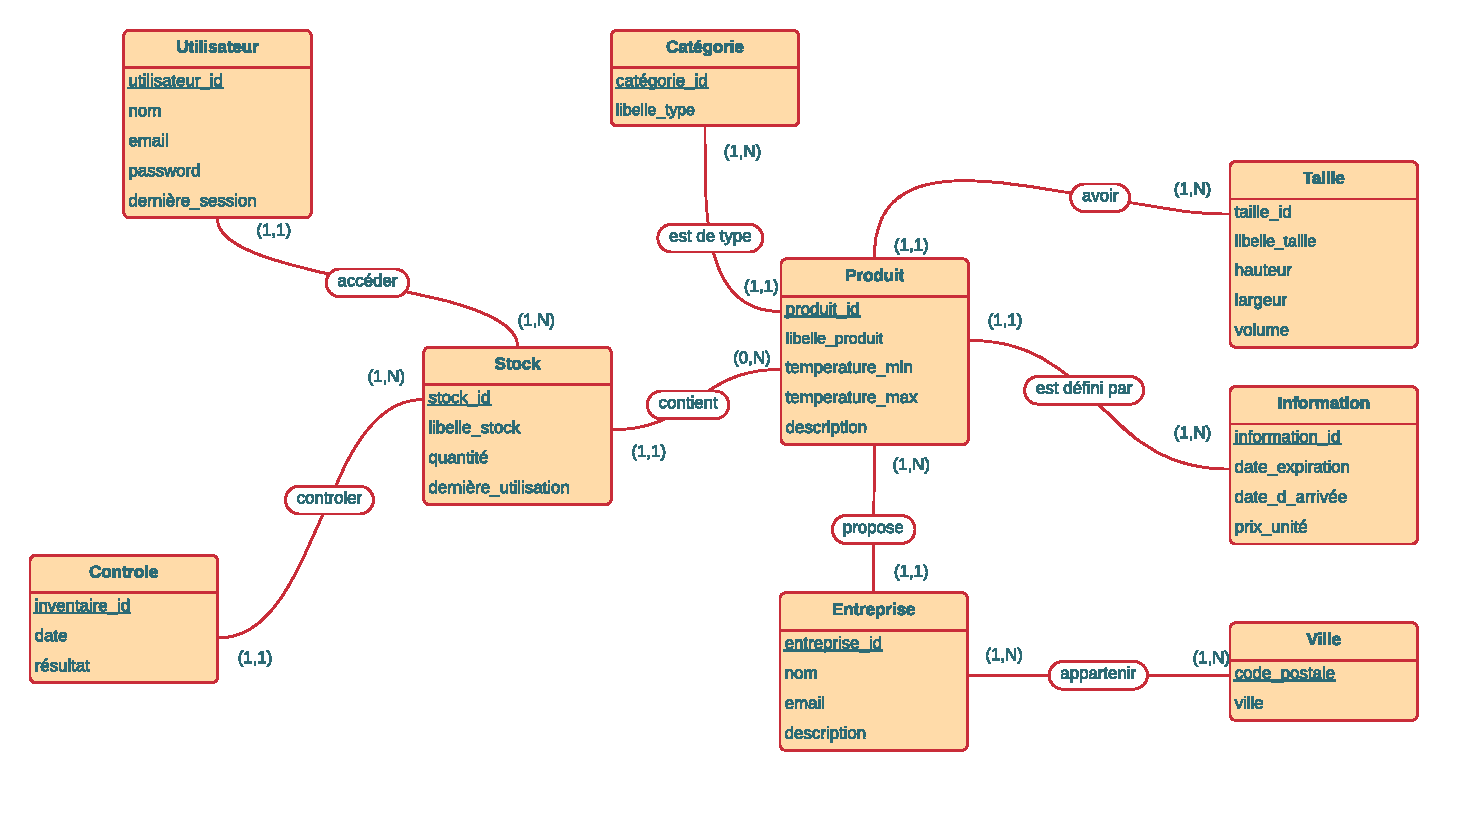
\includegraphics[keepaspectratio=true,scale=0.6]{Figures/mcd.pdf}
    \caption{Modèle EA}
    \label{fig:structure}
\end{figure}

\subsection{Description des entités}
Dans le diagramme entité-association, nous trouvons les entités suivantes :

\paragraph{Ville} Nous savons que chaque ville a son propre et unique code postal. C'est pourquoi nous pouvons le considérer ici comme étant une clé primaire.

\paragraph{Catégorie}
Une catégorie est définie par son identifiant, et son libellé. Nous avons choisi de le considérer comme une entité, au lieu de le mettre comme un attribut dans la table des produits. En effet, il existe de nombreux produits appartenant à la même catégorie (fruits, légumes, viande, etc.…).

\paragraph{Entreprise} Une entreprise est définie par son identifiant, son nom, email, et une brève description.

\paragraph{Utilisateur} Un utilisateur est défini par un identifiant, un nom d'utilisateur et un mot de passe pour accéder à son compte. De plus, pour garder une trace de ses activités, nous avons ajouté la date de la dernière session comme attribut.

\paragraph{Contrôle} Un contrôle est définit par un identifiant, un nom, la date de contrôle, ainsi que le résultat de contrôle.

\paragraph{Stock} Un stock est associé a un et un seul utilisateur. Il est définit par un identifiant unique, et un libellé.

\paragraph{Information} Il contient un certain nombre d'informations génériques et communes à de nombreux objets, comme la température du produit, la date d'expiration, le prix, la quantité, et la date d'entrée.

\paragraph{Taille} Elle fonctionne de la même manière que l'entité : "Information". L'entité "Taille"
contient des informations relatives à la forme géométrique de l'objet (hauteur, poids, volume).

\paragraph{Produit} Chaque produit est acheté auprès une où plusieurs entreprise. Il est définit par un identifiant unique, un libellé, une description, des informations uniques relative au produit comme la température du produit (la plus basse et la plus haute).


\section{Modèle logique de données (MLD)}
\subsection{Modèle relationnel}
Grâce au modèle conceptuel précédent, on a établi le modèle relationnel qui suit :

\paragraph{UTILISATEUR} (\textbf{\underline{utilisateur\_id}}, utilisateur\_nom, utilisateur\_email, utilisateur\_password, utilisateur\_dernière\_session, \#stock\_id)
\paragraph{STOCK} (\textbf{\underline{stock\_id}}, libellé\_stock, \#produit\_id)
\paragraph{CONTRÔLE} (\textbf{\underline{contrôle\_id}}, contrôle\_date, \#stock\_id)
\paragraph{PRODUIT} (\textbf{\underline{produit\_id}}, libellé\_produit, température\_max, température\_min, produit\_description, \#catégorie\_id, \#information\_id, \#taille\_id)
\paragraph{CATÉGORIE } (\textbf{\underline{catégorie\_id}}, libellé\_catégorie)
\paragraph{ENTREPRISE} (\textbf{\underline{entreprise\_id}}, entreprise\_nom, entreprise\_email, entreprise\_description, \#produit\_id)
\paragraph{VILLE} (\textbf{\underline{code\_postale}}, ville)
\paragraph{APPARTENIR} (\textbf{\underline{\#code\_postale, \#entreprise\_id}})
\paragraph{TAILLE} (\textbf{\underline{taille\_id}}, libellé\_taille, taille\_hauteur, taille\_largeur, taille\_volume)
\paragraph{INFORMATION} (\textbf{\underline{information\_id}}, date\_expiration, date\_d\_arrivée, prix\_unité, quantité)

\subsection{Dépendance fonctionnelle}

\begin{table}[H]
\resizebox{1.14\columnwidth}{!}{%
\begin{tabular}{lll}
\textbf{utilisateur\_id}&  $\longrightarrow$ &  \#stock\_id, utilisateur\_nom, utilisateur\_email, utilisateur\_password, \\
&& utilisateur\_dernière\_session \\
&&\\
\textbf{stock\_id}& $\longrightarrow$ & \#produit\_id, libellé\_stock \\
&&\\
\textbf{contrôle\_id}& $\longrightarrow$ & \#stock\_id, contrôle\_date \\
&&\\
\textbf{produit\_id}& $\longrightarrow$ & \#catégorie\_id, \#information\_id, \#taille\_id, libellé\_produit,\\
&& température\_max, température\_min, produit\_description \\
&&\\
\textbf{catégorie\_id}& $\longrightarrow$ & libellé\_catégorie \\
&&\\
\textbf{entreprise\_id}& $\longrightarrow$ & \#produit\_id, entreprise\_nom, entreprise\_email, entreprise\_description \\
&&\\
\textbf{code\_postale}& $\longrightarrow$ & ville \\
&&\\
(\textbf{\#code\_postale, \#entreprise\_id})& $\longrightarrow$ & \textit{évident.} \\
&&\\
\textbf{taille\_id}& $\longrightarrow$ & libellé\_taille, taille\_hauteur, taille\_largeur, taille\_volume \\
&&\\
\textbf{information\_id}& $\longrightarrow$ & date\_expiration, date\_d\_arrivée, prix\_unité, quantité
\end{tabular}
}
\end{table}


\subsection{Normalisation de la base en 3 forme normale}

\paragraph{UTILISATEUR} (\textbf{\underline{utilisateur\_id}}, utilisateur\_nom, utilisateur\_email, utilisateur\_password, utilisateur\_dernière\_session, \#stock\_id)

\texttt{utilisateur\_id} est le clé. En effet, toutes combinaison des attributs : \texttt{utilisateur\_nom, utilisateur\_email} et \texttt{utilisateur\_password} ne permet pas de retrouver les valeurs des autres attributs.

On a la $1^{\text{er}}$ forme normale (FN1). Car, tous les attributs sont atomiques. De plus, on a dépendance totale de la clé principale \texttt{utilisateur\_id}, ainsi, elle est aussi atomique. Donc, on a la $2^{\text{ème}}$ forme normale (FN2). Enfin, aucune combinaison entre les attributs ne suffissent pour déduire les autres attributs. On la $3^{\text{ème}}$ forme normale (FN3).

$\Longrightarrow\:$ \textbf{\textit{FN3 est respectée.}}

\paragraph{STOCK} (\textbf{\underline{stock\_id}}, libellé\_stock, \#produit\_id)

\texttt{stock\_id} est le clé. Car, tous les autres attributs dépendent fonctionnellement du clé \texttt{stock\_id}. Tous les attributs sont atomiques, on a bien la $1^{\text{er}}$ forme normale (FN1).

La clé est simple et non composite, et tous les autres attributs dépendent de la clé. Donc, on a la $2^{\text{ème}}$ forme normale (FN2). Ainsi, aucune combinaison entre les attributs ne suffissent pour déduire les autres attributs. On la $3^{\text{ème}}$ forme normale (FN3).

$\Longrightarrow\:$ \textbf{\textit{FN3 est respectée.}}

\paragraph{CONTRÔLE} (\textbf{\underline{contrôle\_id}}, contrôle\_date, \#stock\_id)

$\Longrightarrow\:$ \textbf{\textit{FN3 est respectée.}}

\paragraph{PRODUIT} (\textbf{\underline{produit\_id}}, libellé\_produit, température\_max, température\_min, produit\_description, \#catégorie\_id, \#information\_id, \#taille\_id)

\texttt{produit\_id} est le clé. Car, tous les autres attributs dépendent fonctionnellement du clé \texttt{produit\_id}. Tous les attributs sont atomiques, on a bien la $1^{\text{er}}$ forme normale (FN1).

La clé est simple et non composite, et tous les autres attributs dépendent de la clé. Donc, on a la $2^{\text{ème}}$ forme normale (FN2). Ainsi, aucune combinaison entre les attributs ne suffissent pour déduire les autres attributs. On la $3^{\text{ème}}$ forme normale (FN3).

$\Longrightarrow\:$ \textbf{\textit{FN3 est respectée.}}

\paragraph{CATÉGORIE } (\textbf{\underline{catégorie\_id}}, libellé\_catégorie)

$\Longrightarrow\:$ \textbf{\textit{FN3 est respectée.}}

\paragraph{ENTREPRISE} (\textbf{\underline{entreprise\_id}}, entreprise\_nom, entreprise\_email, entreprise\_description, \#produit\_id)

\texttt{entreprise\_id} est le clé. Car, tous les autres attributs dépendent fonctionnellement du clé \texttt{entreprise\_id}. Tous les attributs sont atomiques, on a bien la $1^{\text{er}}$ forme normale (FN1). De plus, on a dépendance totale de la clé principale. En effet, le clé est simple (non composite) et tous les autres attributs dépendent de la clé. On a donc le $2^{\text{ème}}$ forme normale (FN2). Enfin, on a $3^{\text{ème}}$ forme normale (FN3). Car, aucune combinaison entre les attributs ne suffissent pour déduire les autres attributs.

$\Longrightarrow\:$ \textbf{\textit{FN3 est respectée.}}



\paragraph{VILLE} (\textbf{\underline{code\_postale}}, ville)

On a la $1^{\text{er}}$ forme normale (FN1). En effet, tous les attributs sont atomiques, et l'identifiant \texttt{code\_postale} est unique. De plus, on a dépendance totale de la clé principale. En effet, le clé est simple (non composite) et l'attribut \texttt{ville} dépend de la clé. On a donc le $2^{\text{ème}}$ forme normale (FN2). On a $3^{\text{ème}}$ forme normale (FN3). Car, l'attribut \texttt{ville} dépend de la clé.

$\Longrightarrow\:$ \textbf{\textit{FN3 est respectée.}}

\paragraph{APPARTENIR} (\textbf{\underline{\#code\_postale, \#entreprise\_id}})

Les deux clés sont atomiques.

$\Longrightarrow\:$ \textbf{\textit{FN3 est respectée.}}é

\paragraph{TAILLE} (\textbf{\underline{taille\_id}}, libellé\_taille, taille\_hauteur, taille\_largeur, taille\_volume)

$\Longrightarrow\:$ \textbf{\textit{FN3 est respectée.}}

\paragraph{INFORMATION} (\textbf{\underline{information\_id}}, date\_expiration, date\_d\_arrivée, prix\_unité, quantité)

$\Longrightarrow\:$ \textbf{\textit{FN3 est respectée.}}

	\chapter{Réalisation} \label{Chapter4}

\section{Introduction}

\section{Environnement de développement}
Il s’agit dans cette partie d’identifier les différentes caractéristiques de l’environnement matériel et logiciel qui nous ont servi à l’implémentation de notre application.

\subsection{Environnement matériel}
La machine utilisée pour réaliser ce site est un ordinateur portable Lenovo qui a la configuration suivante :

\paragraph{Système d’exploitation} Windows 10
\paragraph{Processeur} Intel(R) Core(TM) i7-8550U CPU
\paragraph{Mémoire RAM installée} 8,00 Go

\subsection{Environnement logiciel}
Nous allons maintenant donner une brève définition de chaque langage et bibliothèque utilisés.

\subsection*{Git}
\begin{wrapfigure}{r}{0.30\textwidth} %this figure will be at the right
    \centering
    
\includegraphics[width=0.2\textwidth]{Figures/git.png}
    \caption{Git}
\end{wrapfigure}
Git est un système de contrôle de version. Il conserve un historique de toutes les modifications apportées au code. Les modifications sont stockées dans une base de données spéciale appelée "repository", également connue sous le nom de "repo".

L'utilisation de Git pour le développement de logiciels présente deux avantages principaux :
\begin{itemize}
    \item Le suivi des modifications et des mises à jour. On est capable de voir qui a fait quels changements. Git permet également de savoir quand et pourquoi un changement a été effectué.
    \item Permettre de travailler en collaboration. Les projets de développement de logiciels nécessitent généralement que de nombreuses personnes travaillent ensemble. Git fournit aux développeurs un moyen systématique de le faire. Ainsi, les développeurs se concentrent sur le projet plutôt que sur les longues sessions de communication entre les autres développeurs.
    \item Il existe d'autres systèmes de contrôle de version, tels que Subversion, Mercurial, etc. Cependant, Git est le plus populaire.
\end{itemize}

Pendant le processus de réalisation, nous utiliserons la plateforme GiHub.

\subsection*{Python}
\begin{wrapfigure}{r}{0.30\textwidth} %this figure will be at the right
    \centering
    
\includegraphics[width=0.15\textwidth]{Figures/python.png}
    \caption{Python}
\end{wrapfigure}
Python est un langage de programmation open-source, interprété, orienté objet, de haut niveau avec une sémantique dynamique, avec des applications dans de nombreux domaines, notamment la programmation web, les scripts, le calcul scientifique et l'intelligence artificielle. Il est bien structuré et nombre de ses fonctionnalités prennent en charge la programmation fonctionnelle, la méta programmation et les méta-objets.

Il est très populaire et largement utilisé par des organisations connues telles que la NASA et Google, entre autres.


\subsection*{La bibliothèque \texttt{mysql-connector-python}}
\begin{wrapfigure}{r}{0.30\textwidth} %this figure will be at the right
    \centering
    
\includegraphics[width=0.20\textwidth]{Figures/mysql.png}
    \caption{mysql-connector-python}
\end{wrapfigure}
MySQL est un système de gestion de bases de données relationnelles (SGBDR) open source et gratuit qui utilise le langage de requête structuré (SQL).
Dans cet article, nous allons partager une explication complète sur MySQL. Il s'agit d'un système de gestion de base de données relationnelle (SGBDR) open-source avec un modèle client-serveur.  Un SGBDR est un logiciel ou un service utilisé pour créer et gérer des bases de données basées sur un modèle relationnel.

Nous avons décidé dans ce projet d'utiliser python au lieu du langage Java, pour la simplicité et la disponibilité de la bibliothèque \texttt{mysql-connector-python}.

\section{Création de la base de données}
\begin{lstlisting}[
    language=SQL,
    showspaces=false,
    basicstyle=\ttfamily,
    numbers=left,
    numberstyle=\tiny,
    commentstyle=\color{gray}
]
--
-- Database : Home
--
DROP DATABASE IF EXISTS Home;
CREATE DATABASE IF NOT EXISTS Home;
USE Home;
\end{lstlisting}

\subsection{Création des tables de la base de données}
\subsubsection*{Utilisateur}
\begin{lstlisting}[
    language=SQL,
    showspaces=false,
    basicstyle=\ttfamily,
    numbers=left,
    numberstyle=\tiny,
    commentstyle=\color{gray}
]
--
-- Structure de la table : utilisateur
--
DROP TABLE IF EXISTS user;
CREATE TABLE IF NOT EXISTS user (
    user_id INT NOT NULL AUTO_INCREMENT,
    user_name VARCHAR(50) NOT NULL,
    user_password VARCHAR(50) NOT NULL,
    user_last_session DATETIME NOT NULL,

    PRIMARY KEY (user_id)
);
\end{lstlisting}

\subsubsection*{Ville}
\begin{lstlisting}[
    language=SQL,
    showspaces=false,
    basicstyle=\ttfamily,
    numbers=left,
    numberstyle=\tiny,
    commentstyle=\color{gray}
]
--
-- Structure de la table : City
--
DROP TABLE IF EXISTS City;
CREATE TABLE IF NOT EXISTS City (
    zip_code INT NOT NULL AUTO_INCREMENT,

    city_name VARCHAR(50) NOT NULL,

    PRIMARY KEY (zip_code)
);
\end{lstlisting}

\subsubsection*{Catégorie}
\begin{lstlisting}[
    language=SQL,
    showspaces=false,
    basicstyle=\ttfamily,
    numbers=left,
    numberstyle=\tiny,
    commentstyle=\color{gray}
]
--
-- Structure de la table : Category
--
DROP TABLE IF EXISTS Category;
CREATE TABLE IF NOT EXISTS Category (
    category_id INT NOT NULL AUTO_INCREMENT,

    category_nom VARCHAR(50) NOT NULL,

    PRIMARY KEY (category_id)
);
\end{lstlisting}

\subsubsection*{Entreprise}
\begin{lstlisting}[
    language=SQL,
    showspaces=false,
    basicstyle=\ttfamily,
    numbers=left,
    numberstyle=\tiny,
    commentstyle=\color{gray}
]
--
-- Structure de la table : Company
--
DROP TABLE IF EXISTS Company;
CREATE TABLE IF NOT EXISTS Company (
    company_id INT NOT NULL AUTO_INCREMENT,

    product_id INT NOT NULL,

    company_name VARCHAR(50) NOT NULL,
    company_email VARCHAR(50) NOT NULL,
    company_description VARCHAR(50) NOT NULL,

    PRIMARY KEY (company_id),
    FOREIGN KEY (product_id) REFERENCES Product(product_id)
);
\end{lstlisting}

\subsubsection*{Contrôle}
\begin{lstlisting}[
    language=SQL,
    showspaces=false,
    basicstyle=\ttfamily,
    numbers=left,
    numberstyle=\tiny,
    commentstyle=\color{gray}
]
--
-- Structure de la table : Control
--
DROP TABLE IF EXISTS Control;
CREATE TABLE IF NOT EXISTS Control (
    control_id INT NOT NULL AUTO_INCREMENT,

    stock_id INT NOT NULL,

    control_date DATETIME NOT NULL,

    PRIMARY KEY (control_id),
    FOREIGN KEY (stock_id) REFERENCES Stock(stock_id)
);
\end{lstlisting}

\subsubsection*{Stock}
\begin{lstlisting}[
    language=SQL,
    showspaces=false,
    basicstyle=\ttfamily,
    numbers=left,
    numberstyle=\tiny,
    commentstyle=\color{gray}
]
--
-- Structure de la table : Stock
--
DROP TABLE IF EXISTS Stock;
CREATE TABLE IF NOT EXISTS Stock (
    stock_id INT NOT NULL AUTO_INCREMENT,

    product_id INT NOT NULL,

    stock_name VARCHAR(50) NOT NULL,

    PRIMARY KEY (stock_id),
    FOREIGN KEY (product_id) REFERENCES Product(product_id)
);
\end{lstlisting}

\subsubsection*{Information}
\begin{lstlisting}[
    language=SQL,
    showspaces=false,
    basicstyle=\ttfamily,
    numbers=left,
    numberstyle=\tiny,
    commentstyle=\color{gray}
]
--
-- Structure de la table : Information
--
DROP TABLE IF EXISTS Information;
CREATE TABLE IF NOT EXISTS Information (
    information_id INT NOT NULL AUTO_INCREMENT,

    information_expiration_date DATETIME NOT NULL,
    information_entry_date DATETIME NOT NULL,
    information_unit_price INT NOT NULL,
    information_quantity INT NOT NULL,

    PRIMARY KEY (information_id)
);
\end{lstlisting}

\subsubsection*{Taille}
\begin{lstlisting}[
    language=SQL,
    showspaces=false,
    basicstyle=\ttfamily,
    numbers=left,
    numberstyle=\tiny,
    commentstyle=\color{gray}
]
--
-- Structure de la table : Shape
--
DROP TABLE IF EXISTS Shape;
CREATE TABLE IF NOT EXISTS Shape (
    shape_id INT NOT NULL AUTO_INCREMENT,

    shape_name VARCHAR(50) NOT NULL,
    shape_height VARCHAR(50) NOT NULL,
    shape_weight VARCHAR(50) NOT NULL,
    shape_volume VARCHAR(50) NOT NULL,

    PRIMARY KEY (shape_id)
);
\end{lstlisting}

\subsubsection*{Produit}
\begin{lstlisting}[
    language=SQL,
    showspaces=false,
    basicstyle=\ttfamily,
    numbers=left,
    numberstyle=\tiny,
    commentstyle=\color{gray}
]
--
-- Structure de la table : Product
--
DROP TABLE IF EXISTS Product;
CREATE TABLE IF NOT EXISTS Product (
    product_id INT NOT NULL AUTO_INCREMENT,

    shape_id INT NOT NULL,
    information_id INT NOT NULL,
    category_id INT NOT NULL,

    product_name VARCHAR(50) NOT NULL,
    product_temperature_max VARCHAR(50) NOT NULL,
    product_temperature_min VARCHAR(50) NOT NULL,
    product_description VARCHAR(50) NOT NULL,

    PRIMARY KEY (product_id),
    FOREIGN KEY (shape_id) REFERENCES Shape(shape_id),
    FOREIGN KEY (information_id) REFERENCES Information(information_id),
    FOREIGN KEY (category_id) REFERENCES Category(category_id)
);
\end{lstlisting}

\subsubsection*{Appartenir}
\begin{lstlisting}[
    language=SQL,
    showspaces=false,
    basicstyle=\ttfamily,
    numbers=left,
    numberstyle=\tiny,
    commentstyle=\color{gray}
]
--
-- Structure de la table : BELONGING
--
DROP TABLE IF EXISTS BELONGING;
CREATE TABLE IF NOT EXISTS BELONGING (
    zip_code INT NOT NULL,
    company_id INT NOT NULL,

    FOREIGN KEY (zip_code) REFERENCES City(zip_code),
    FOREIGN KEY (company_id) REFERENCES Company(company_id),
    CONSTRAINT PRIMARY KEY (
        zip_code,
        company_id
    )
);
\end{lstlisting}

\subsection{Contraintes d'intégrité}
\begin{lstlisting}[
    language=SQL,
    showspaces=false,
    basicstyle=\ttfamily,
    numbers=left,
    numberstyle=\tiny,
    commentstyle=\color{gray}
]
--
-- Contraintes d'intégrité
--

ALTER TABLE Product
ADD CONSTRAINT
    CHECK (
        product_temperature_max > 0 AND
        product_temperature_min > 0
    );

ALTER TABLE Shape
ADD CONSTRAINT
    CHECK (
        shape_height > 0 AND
        shape_weight > 0 AND
        shape_volume > 0 AND
    );

ALTER TABLE Information
ADD CONSTRAINT
    CHECK (
        information_quantity > 0 AND
        information_entry_date <= information_expiration_date AND
        information_unit_price > 0
    );

ALTER TABLE Control
MODIFY control_results ENUM (
    'Produit est périmé',
    'Produit est disponible',
    'Produit n est pas disponile'
);
\end{lstlisting}

\subsection{Commandes SQL}
Cette partie a pour objectif : tester toutes les requêtes avant de les ajouter dans le code permettant de contrôler l’application.

\subsubsection{Requêtes concernant l'affichage d'un produit}
\begin{lstlisting}[
    language=SQL,
    showspaces=false,
    basicstyle=\ttfamily,
    numbers=left,
    numberstyle=\tiny,
    commentstyle=\color{gray}
]
SELECT product_name, category_name
FROM Product, Category
WHERE Product.category_id = Category.category_id;
\end{lstlisting}


\subsubsection{Requêtes concernant l'affichage de derniers résultats de contrôle des produits}
\begin{lstlisting}[
    language=SQL,
    showspaces=false,
    basicstyle=\ttfamily,
    numbers=left,
    numberstyle=\tiny,
    commentstyle=\color{gray}
]
SELECT product_name, control_results
FROM Product, Control, Stock
Where
	Control.stock_id = Stock.stock_id AND
    Stock.product_id = Product.product_id
GROUP by product_name;
\end{lstlisting}


\subsubsection{Requêtes concernant modification de mot de passe}
\begin{lstlisting}[
    language=SQL,
    showspaces=false,
    basicstyle=\ttfamily,
    numbers=left,
    numberstyle=\tiny,
    commentstyle=\color{gray}
]
UPDATE User
SET
    user_password = password
WHERE
    user_name = name;
\end{lstlisting}

\subsubsection{Requêtes concernant la suppression d'un produit}
\begin{lstlisting}[
    language=SQL,
    showspaces=false,
    basicstyle=\ttfamily,
    numbers=left,
    numberstyle=\tiny,
    commentstyle=\color{gray}
]
DELETE FROM User
WHERE product_name = name
\end{lstlisting}

\section{Interfaces}

\begin{figure}[ht!]
    \centering
    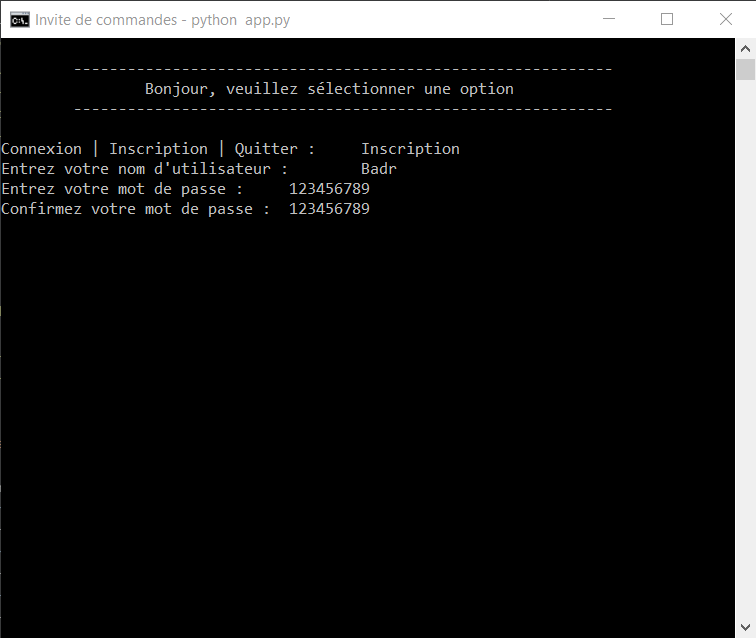
\includegraphics[keepaspectratio=true,scale=0.7]{Figures/img1.png}
    \caption{Ouvrir un compte}
    \label{fig:img1}
\end{figure}

\begin{figure}[ht!]
    \centering
    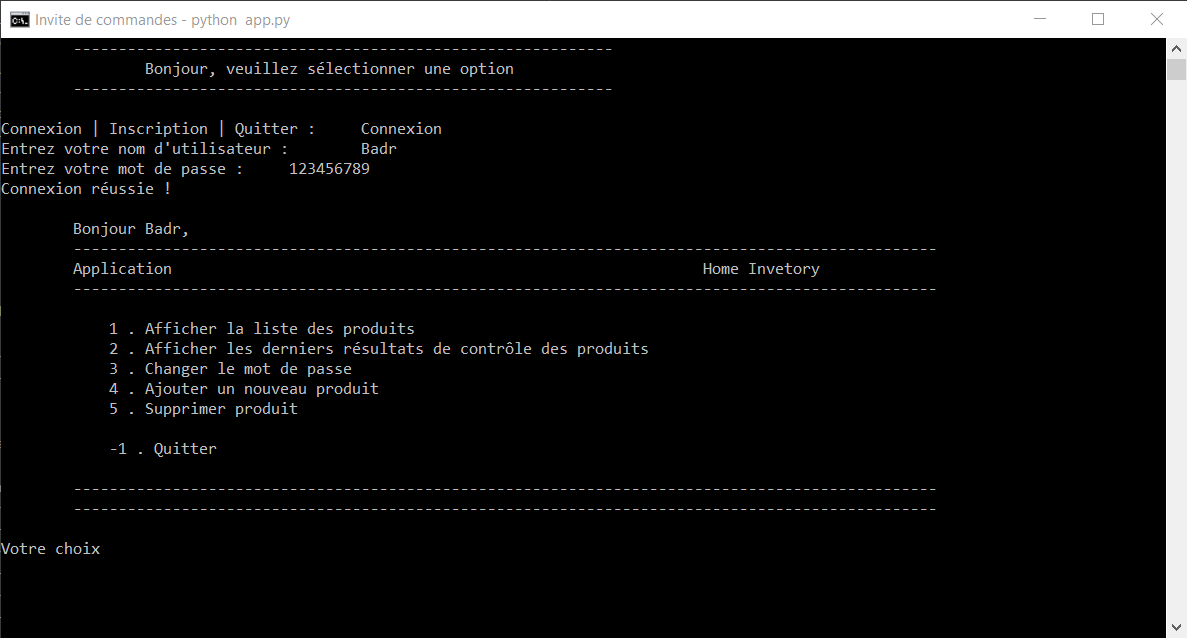
\includegraphics[keepaspectratio=true,scale=0.7]{Figures/img2.png}
    \caption{Page d'accueil}
    \label{fig:img1}
\end{figure}

\begin{figure}[ht!]
    \centering
    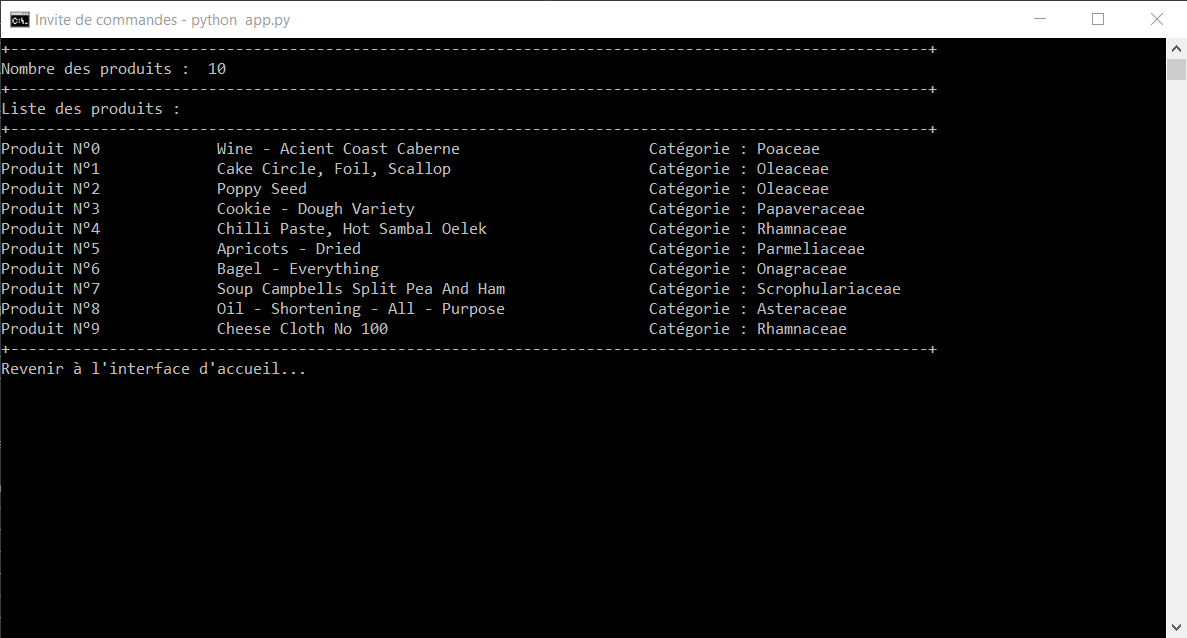
\includegraphics[keepaspectratio=true,scale=0.7]{Figures/img3.png}
    \caption{Liste des produits}
    \label{fig:img1}
\end{figure}

\begin{figure}[ht!]
    \centering
    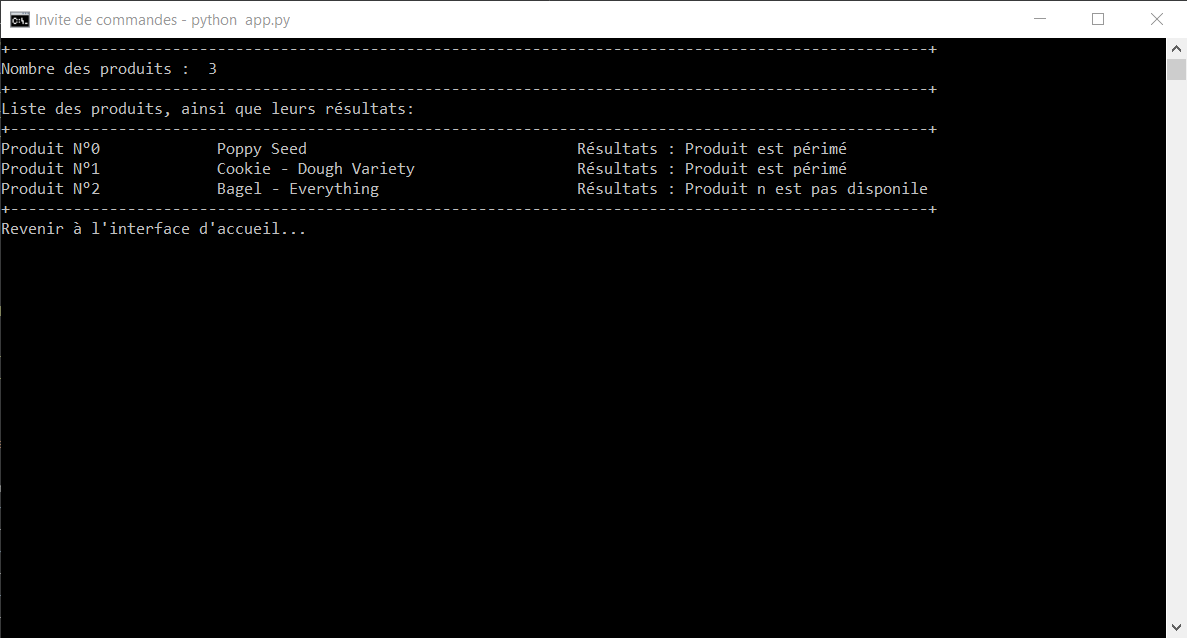
\includegraphics[keepaspectratio=true,scale=0.7]{Figures/img4.png}
    \caption{Liste des résultats de contrôle}
    \label{fig:img1}
\end{figure}

	\chapter{Conclusion générale} \label{Chapter5}

Les cours de base de données et ce projet nous a été très utile pour bien comprendre tout les notions vues ce semestre : conception et analyse avec création du modèle conceptuel puis traduction en modèle relationnel, et ensuite la réalisation avec la création de la base de données.

L’expérience était réussie pour tous les membres de l’équipe parce que nous étions obligés d’aller chercher et explorer d’autres méthodes et outils pour résoudre notre problème d’aller plus loin dans l’analyse.


	\appendix
    % Appendix Template

\chapter{Code Python} \label{annexe1}

Tous les programmes sont disponibles sur la plateforme github.

\section{Fichier \texttt{auth.py}}

\begin{lstlisting}[
    language=Python
    showspaces=false,
    basicstyle=\ttfamily,
    basicstyle=\tiny,
    numbers=left,
    numberstyle=\tiny,
]
import mysql.connector
import os
import time

from app.interface import home


connection = mysql.connector.connect(
    host = 'localhost',
    port = '3306',
    database = 'Home',
    user = 'root',
    password = 'toor'
)
cursor = connection.cursor()

def gain_access(Username=None, Password=None):

    Username = str(input("Entrez votre nom d'utilisateur :\t"))
    Password = str(input("Entrez votre mot de passe :\t"))

    if not len(Username or Password) < 1:
        if True:
            cursor.execute('SELECT user_name, user_password FROM User')
            data = cursor.fetchall()
            if (Username, Password) in data :
                print("Connexion réussie !")
                time.sleep(1)
                home(Username)
            else :
                print("Le mot de passe ou le nom d'utilisateur n'existe pas")
        else:
            print("Erreur de connexion au système")

    else:
        print("Veuillez essayer de vous connecter à nouveau.")
        os.system('cls'); gain_access()

def register(Username=None, Password1=None, Password2=None):
    Username = input("Entrez votre nom d'utilisateur :\t")
    Password1 = input("Entrez votre mot de passe :\t")
    Password2 = input("Confirmez votre mot de passe :\t")


    if not len(Password1) <= 6:
        if not Username == None:
            if len(Username) < 1:
                print("Veuillez fournir un nom d'utilisateur")
                time.sleep(1); os.system('cls');
                register()
            else:
                if Password1 == Password2:

                    cursor.execute("insert into user (user_name, user_password, stock_id) values (%s, %s, 2)", (Username, Password1))
                    connection.commit()

                    print("Utilisateur créé avec succès !")
                    print("Veuillez vous connecter pour continuer...")
                    time.sleep(1); os.system('cls');
                    gain_access()

                else:
                    print("Les mots de passe ne sont pas identiques")
                    time.sleep(1); os.system('cls');
                    register()
    else:
        print("Mot de passe trop court")
        time.sleep(1); os.system('cls');
        register()
\end{lstlisting}

\section{Fichier \texttt{home\_app.py}}


\begin{lstlisting}[
    language=Python
    showspaces=false,
    basicstyle=\ttfamily,
    basicstyle=\tiny,
    numbers=left,
    numberstyle=\tiny,
]
import mysql.connector
import time
import os

connection = mysql.connector.connect(
    host = 'localhost',
    port = '3306',
    database = 'Home',
    user = 'root',
    password = 'toor'
)
cursor = connection.cursor()

def print_products() :
    cursor.execute("""
        SELECT product_name, category_name
        FROM Product, Category
        Where Product.category_id = Category.category_id
    """)
    data = cursor.fetchall()

    print("Nombre des produits : ", len(data))
    print("Liste des produits :")
    i = 0
    for d in data :
        print("Produit N°{:<12}\t{:<35}\t\tCatégorie : {:<12}".format(i, d[0], d[1]), end='\n'); i += 1

    if input("Revenir à l'interface d'accueil...") != '' :
        os.system('cls');


def print_results() :
    cursor.execute("""
        SELECT product_name, control_results
        FROM Product, Control, Stock
        Where
        	Control.stock_id = Stock.stock_id AND
            Stock.product_id = Product.product_id
        GROUP by product_name
    """)
    data = cursor.fetchall()

    print("Nombre des produits : ", len(data))
    print("Liste des produits, ainsi que leurs résultats:")
    i = 0
    for d in data :
        print("Produit N°{:<12}\t{:<30}\t\tRésultats : {:<12}".format(i, d[0], d[1]), end='\n'); i += 1

    if input("Revenir à l'interface d'accueil...") != '' :
        os.system('cls');

def change_password(Username = None) :
    Password1 = input("Entrez votre mot de passe :\t")
    Password2 = input("Confirmez votre mot de passe :\t")

    if Password1 == Password2 :

        cursor.execute("""
            UPDATE User
            SET
                user_password = {}
            WHERE
                user_name = {};
        """.format(Username, Password1))
        connection.commit()

        print("Mot de passe changée avec succès !")

    if input("Revenir à l'interface d'accueil...") != '' :
        os.system('cls');

def delete_product() :
    name = input("Entrez le nom de produit :\t")

    cursor.execute("""
        DELETE FROM User
        WHERE product_name = {}
    """.format(name))
    connection.commit()

    print("Produit supprimée avec succès !")


def add_new_product() :
    name = input("Entrez le nom de produit :\t")
    taille = input("Entrez le libellé de sa taille :\t")
    temp_min = input("Entrez sa temperature minimal :\t")
    temp_max = input("Entrez sa temperature maximal :\t")
    desc = input("Entrez une description de produit :\t")

    cursor.execute("""
        insert into Product
            (product_name, product_temperature_max, product_temperature_min, product_description, shape_id, information_id, category_id) values
            ({}, {}, {}, {}, {}, {}, {});
    """.format(name, taille, temp_min, temp_max, desc, 1, 1, 1))
    connection.commit()


    print("Mot de passe ajoutée avec succès !")


    if input("Revenir à l'interface d'accueil...") != '' :
        os.system('cls');

\end{lstlisting}

    \chapter{Structure des tables en MySQL}
\begin{landscape}
\begin{lstlisting}[
  language   = SQL,
  basicstyle = \tiny\ttfamily,
  columns    = fixed,
]
mysql> describe User;
+-------------------+-------------+------+-----+---------+----------------+
| Field             | Type        | Null | Key | Default | Extra          |
+-------------------+-------------+------+-----+---------+----------------+
| user_id           | int         | NO   | PRI | NULL    | auto_increment |
| stock_id          | int         | NO   | MUL | NULL    |                |
| user_name         | varchar(50) | NO   |     | NULL    |                |
| user_password     | varchar(50) | NO   |     | NULL    |                |
| user_last_session | datetime    | YES  |     | NULL    |                |
+-------------------+-------------+------+-----+---------+----------------+
5 rows in set (0.08 sec)

mysql> describe product;
+-------------------------+-------------+------+-----+---------+----------------+
| Field                   | Type        | Null | Key | Default | Extra          |
+-------------------------+-------------+------+-----+---------+----------------+
| product_id              | int         | NO   | PRI | NULL    | auto_increment |
| shape_id                | int         | NO   | MUL | NULL    |                |
| information_id          | int         | NO   | MUL | NULL    |                |
| category_id             | int         | NO   | MUL | NULL    |                |
| product_name            | varchar(50) | NO   |     | NULL    |                |
| product_temperature_max | varchar(50) | NO   |     | NULL    |                |
| product_temperature_min | varchar(50) | NO   |     | NULL    |                |
| product_description     | varchar(50) | NO   |     | NULL    |                |
+-------------------------+-------------+------+-----+---------+----------------+
8 rows in set (0.24 sec)

mysql> describe category;
+---------------+-------------+------+-----+---------+----------------+
| Field         | Type        | Null | Key | Default | Extra          |
+---------------+-------------+------+-----+---------+----------------+
| category_id   | int         | NO   | PRI | NULL    | auto_increment |
| category_name | varchar(50) | NO   |     | NULL    |                |
+---------------+-------------+------+-----+---------+----------------+
2 rows in set (0.11 sec)

mysql> describe shape;
+--------------+-------------+------+-----+---------+----------------+
| Field        | Type        | Null | Key | Default | Extra          |
+--------------+-------------+------+-----+---------+----------------+
| shape_id     | int         | NO   | PRI | NULL    | auto_increment |
| shape_name   | varchar(50) | NO   |     | NULL    |                |
| shape_height | varchar(50) | NO   |     | NULL    |                |
| shape_weight | varchar(50) | NO   |     | NULL    |                |
| shape_volume | varchar(50) | NO   |     | NULL    |                |
+--------------+-------------+------+-----+---------+----------------+
5 rows in set (0.04 sec)

mysql> describe information;
+-----------------------------+----------+------+-----+---------+----------------+
| Field                       | Type     | Null | Key | Default | Extra          |
+-----------------------------+----------+------+-----+---------+----------------+
| information_id              | int      | NO   | PRI | NULL    | auto_increment |
| information_expiration_date | datetime | NO   |     | NULL    |                |
| information_entry_date      | datetime | NO   |     | NULL    |                |
| information_unit_price      | int      | NO   |     | NULL    |                |
| information_quantity        | int      | NO   |     | NULL    |                |
+-----------------------------+----------+------+-----+---------+----------------+
5 rows in set (0.00 sec)

mysql> describe company;
+---------------------+-------------+------+-----+---------+----------------+
| Field               | Type        | Null | Key | Default | Extra          |
+---------------------+-------------+------+-----+---------+----------------+
| company_id          | int         | NO   | PRI | NULL    | auto_increment |
| product_id          | int         | NO   | MUL | NULL    |                |
| company_name        | varchar(50) | NO   |     | NULL    |                |
| company_email       | varchar(50) | NO   |     | NULL    |                |
| company_description | varchar(50) | NO   |     | NULL    |                |
+---------------------+-------------+------+-----+---------+----------------+
5 rows in set (0.02 sec)

mysql> describe city;
+-----------+-------------+------+-----+---------+----------------+
| Field     | Type        | Null | Key | Default | Extra          |
+-----------+-------------+------+-----+---------+----------------+
| zip_code  | int         | NO   | PRI | NULL    | auto_increment |
| city_name | varchar(50) | NO   |     | NULL    |                |
+-----------+-------------+------+-----+---------+----------------+
2 rows in set (0.00 sec)

mysql> describe control;
+-----------------+-----------------------------------------------------------------------------------+------+-----+---------+----------------+
| Field           | Type                                                                              | Null | Key | Default | Extra          |
+-----------------+-----------------------------------------------------------------------------------+------+-----+---------+----------------+
| control_id      | int                                                                               | NO   | PRI | NULL    | auto_increment |
| stock_id        | int                                                                               | NO   | MUL | NULL    |                |
| control_date    | datetime                                                                          | NO   |     | NULL    |                |
| control_results | enum('Produit est périmé','Produit est disponible','Produit n est pas disponile') | YES  |     | NULL    |                |
+-----------------+-----------------------------------------------------------------------------------+------+-----+---------+----------------+
4 rows in set (0.00 sec)

mysql> describe belonging;
+------------+------+------+-----+---------+-------+
| Field      | Type | Null | Key | Default | Extra |
+------------+------+------+-----+---------+-------+
| zip_code   | int  | NO   | PRI | NULL    |       |
| company_id | int  | NO   | PRI | NULL    |       |
+------------+------+------+-----+---------+-------+
2 rows in set (0.00 sec)
\end{lstlisting}
\end{landscape}


\end{document}
